\chapter{Método experimental}\label{cha:metodo_experimental}

\AddToShipoutPictureBG*{\put(0,0){%
        \parbox[b][\paperheight]{\paperwidth}{%
            \vfill
            \centering
            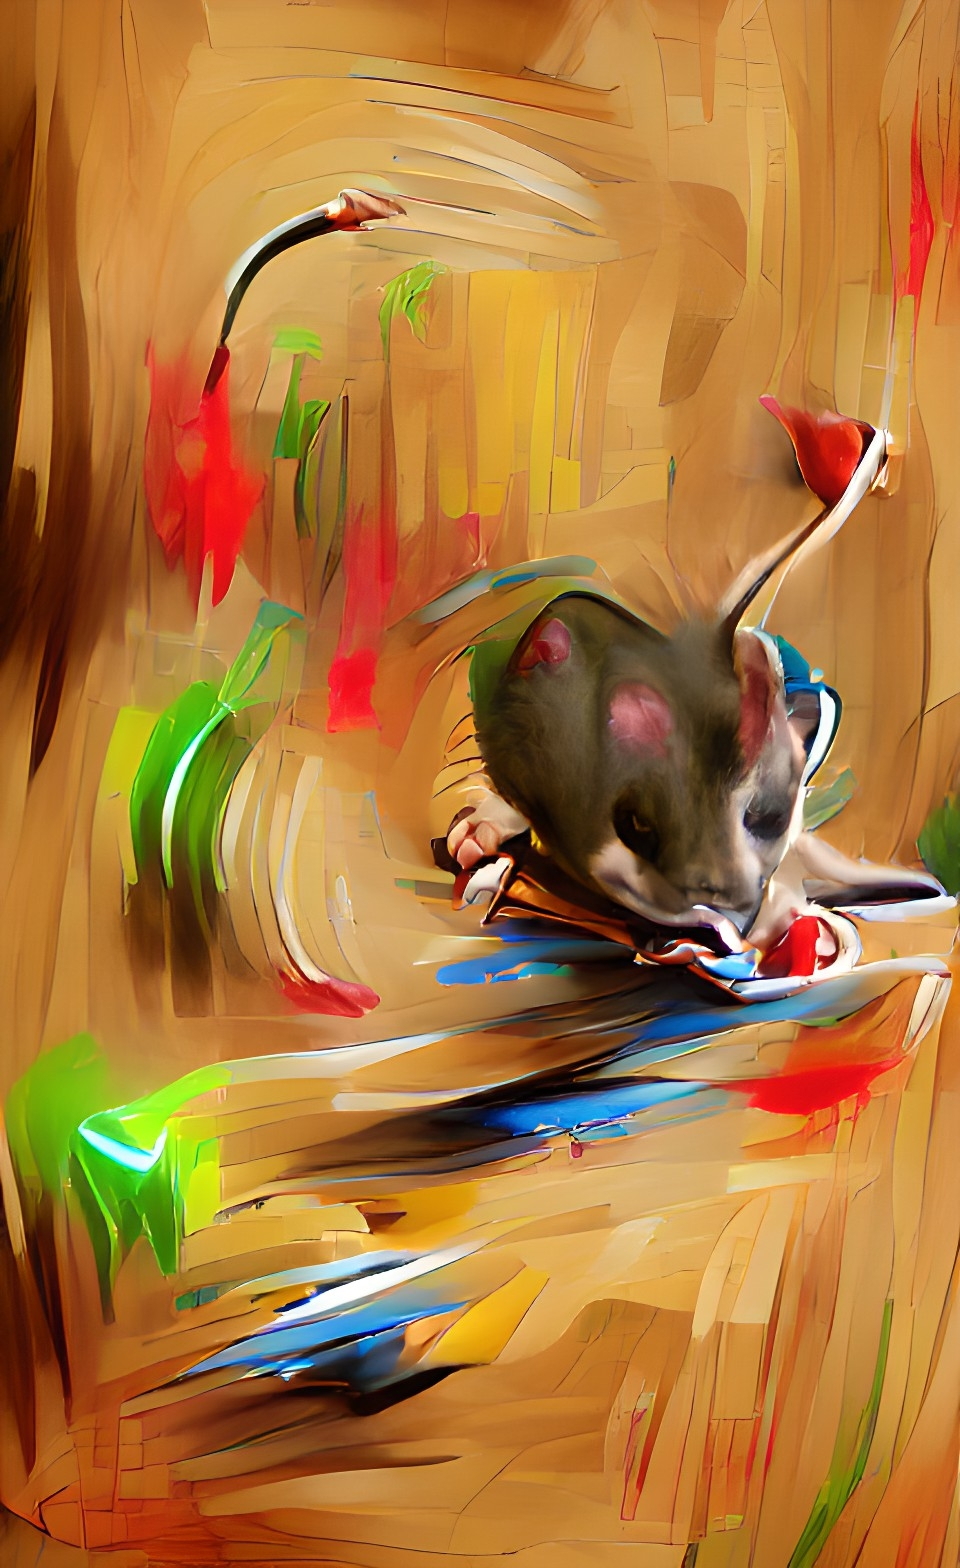
\includegraphics[width=\paperwidth,height=\paperheight,keepaspectratio]{%
                figuras/caratulas/metodo_experimental.jpg}\vfill
        }}}

\AddToShipoutPicture*{
    \begin{tikzpicture}[overlay, remember picture]
        \fill[white, opacity=0.75] (20, 24) rectangle (1, 21);
    \end{tikzpicture}}

\clearpage

Tradicionalmente, predominan dos enfoques a la hora de diseñar experimentos comportamentales en neurociencia. Por un lado, en los estudios de psicología comparada, se analiza el comportamiento como respuesta a estímulos positivos o negativos. Esta perspectiva condujo al desarrollo de trabajos donde los animales se entrenan en el laboratorio para responder a señales sensoriales, recompensas y castigos. Luego, al combinar estos métodos comportamentales con registros y manipulaciones de la actividad neuronal se logra responder preguntas fundamentales sobre cómo están codificadas las variables relacionadas a la tarea comportamental en diferentes regiones del cerebro y qué circuitos neuronales están involucrados. En general, se entrena a los animales para producir acciones relativamente simples (por ejemplo, alcanzar un \textit{pellet} o interactuar con un \textit{lick port}) fáciles de medir y de estudiar junto con patrones de actividad neuronal. Además, suelen utilizarse restricciones físicas para inmovilizar o reducir el movimiento espontáneo de los animales, tanto para facilitar los registros neuronales como para eliminar correlaciones espurias \cite{datta_computational_neuroethology}.

Por otro lado, los estudios etológicos se concentran históricamente en el comportamiento de los animales en entornos naturales \cite{tinbergen_instinct}. La hipótesis subyacente es que exponer la estructura del comportamiento, cómo está compuesto en términos de comportamientos estereotipados y cómo está organizado para responder a estímulos ecológicamente relevantes (es decir, vitales para la supervivencia de la especie y para la adaptación a un entorno) brinda información valiosa sobre cómo el cerebro genera estos comportamientos. Sin embargo, tradicionalmente la etología se concentró en observar el comportamiento animal sin intervenir ni registrar la actividad neuronal. Por lo tanto, explorar la actividad neuronal junto con comportamientos complejos en contextos naturales (por ejemplo, la exploración de nuevos entornos, la obtención de alimento, la búsqueda de refugio o el cortejo, los cuales son comportamientos de iniciativa propia y desarrollados sin mayores restricciones físicas experimentales) tiene el potencial de revelar cómo el cerebro lleva a cabo tareas evolutivamente más importantes. Finalmente, la etología ha mostrado que muchos comportamientos naturales pueden representarse como secuencias de componentes categorizables. En principio, esto permite analizar las relaciones entre las diferentes categorías comportamentales y la actividad neuronal, a lo largo de múltiples escalas temporales y diferentes niveles de detalle en la descripción comportamental \cite{datta_computational_neuroethology, anderson_toward_a_science}.

\clearpage

\begin{figure}[htbp]
    \centering
    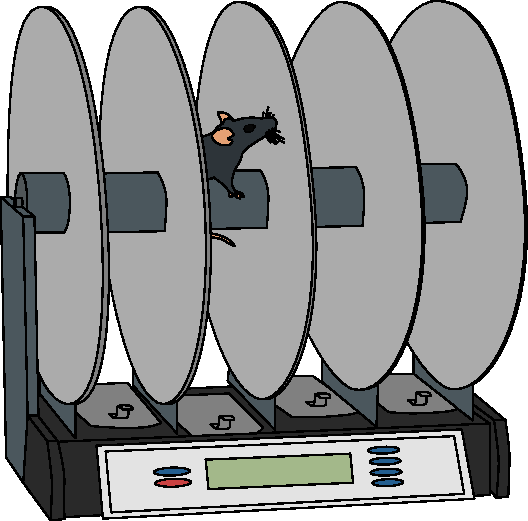
\includegraphics[width=0.5\linewidth]{figuras/capitulo1/rotarod.pdf}
    \caption{\textbf{Aparato rotarod.} El aparato consiste en una varilla rotatoria, compartimentalizada en varias secciones. Un ratón se coloca en una de estas secciones y debe caminar sobre el cilindro que gira a velocidades crecientes.}
    \label{fig:capitulo1_rotarod}
\end{figure}

\section{Protocolo rotarod con aceleración}\label{sec:protocolo}

En este trabajo estudiamos el comportamiento de ratones durante el aprendizaje de la tarea rotarod con aceleración (\autoref{fig:capitulo1_rotarod}). El aparato rotarod está compuesto por una varilla rotatoria, elevada por medio de soportes laterales (\autoref{fig:capitulo1_rotarod}). La elevación de la varilla sirve para desalentar que los ratones salten voluntariamente desde la varilla hacia la mesada, interrumpiendo el correcto desarrollo de la prueba \cite{mouse_tests}. La varilla está compartimentalizada en varias secciones, en principio para poder evaluar a múltiples ratones en paralelo. En la práctica, sin embargo, cada prueba se lleva a cabo con un único ratón por vez sobre el cilindro. Esto se debe a que la presencia de múltiples ratones sobre el cilindro influye en sus comportamientos individuales. El cilindro tiene un diámetro de 3 cm y cada compartimiento del rotarod tiene un ancho de 5.7 cm.

El protocolo de entrenamiento de los ratones consiste en 2 etapas:
\begin{itemize}
    \item La primera etapa abarca 1 o 2 días de habituación antes de dar inicio a la etapa de entrenamiento propiamente dicha. Antes de iniciar las sesiones de entrenamiento (pruebas), los animales son habituados al experimentador y al ambiente del experimento (es decir, a la sala donde se encuentra el aparato rotarod). En esta etapa, los ratones son trasladados a la sala de experimentación y expuestos al rotarod, fuera de funcionamiento, durante un intervalo de tiempo de entre 10 a 15 minutos.

    \item La segunda etapa corresponde al entrenamiento \textit{per se} y es la etapa que se registra en video para posterior análisis. Cada uno de los 10 ratones estudiados se entrena durante 5 días consecutivos. Cada día de entrenamiento consiste en 5 pruebas sucesivas de rotarod, separadas entre sí por 5 minutos de descanso. Las pruebas se llevan a cabo de manera regular durante la mañana, para reducir factores que confundan con el ritmo circadiano de un mismo ratón. En cada prueba el animal es colocado sobre el cilindro rotarod, que gira a velocidades crecientes con aceleración constante, desde 5 rpm hasta 50 rpm en 5 minutos. La prueba termina cuando transcurren un máximo de 5 minutos o cuando el ratón se cae del cilindro. El tiempo transcurrido hasta el fin de la prueba se denomina latencia a caer, y es una métrica clásica para evaluar rendimiento y aprendizaje motor.
\end{itemize}

Originalmente, al aparato rotarod fue diseñado para realizar mediciones automatizadas de déficit neurológico e impedimento motor en roedores, y es actualmente uno de los métodos más comunes para evaluar rendimiento y aprendizaje motor \cite{dunham_rotarod, mouse_tests}. En cuanto a su complejidad, los comportamientos exhibidos en esta tarea están entre los comportamientos sencillos de los experimentos altamente restringidos de la psicología comparada y los comportamientos complejos observados en entornos naturales de la etología. Específicamente, en la tarea rotarod existen restricciones sobre el desplazamiento y la velocidad del ratón, ya que debe caminar sobre un cilindro de dimensiones finitas a una velocidad controlada experimentalmente. Sin embargo, la manera en que el ratón se adapta a estas restricciones biomecánicas es no trivial y varía entre individuos y a lo largo del entrenamiento. Por este motivo, consideramos a la tarea rotarod como ecológicamente relevante, respecto del aprendizaje motor. Principalmente porque expone la manera en que el ratón se adapta a un nuevo entorno y muestra los cambios que sufre su estrategia comportamental para resolver la tarea, siendo esta adaptabilidad a nuevos entornos una habilidad crucial para la supervivencia.

\section{Registros en video}\label{sec:video}

Cada una de las pruebas realizadas se registra en video usando un arreglo de 2 cámaras digitales (\autoref{fig:capitulo1_camaras}). Cada cámara tiene una frecuencia de muestreo de 100 Hz (resolución temporal de 10 ms), capturando fotogramas de 480 px de alto por 640 px de ancho. Por su parte, la cámara frontal captura los movimientos de la cabeza, de las patas delanteras y de parte del lomo del ratón, mientras que la cámara trasera filma los movimientos caudales, de las patas traseras y del lomo del ratón.

\begin{figure}[htbp]
    \centering
    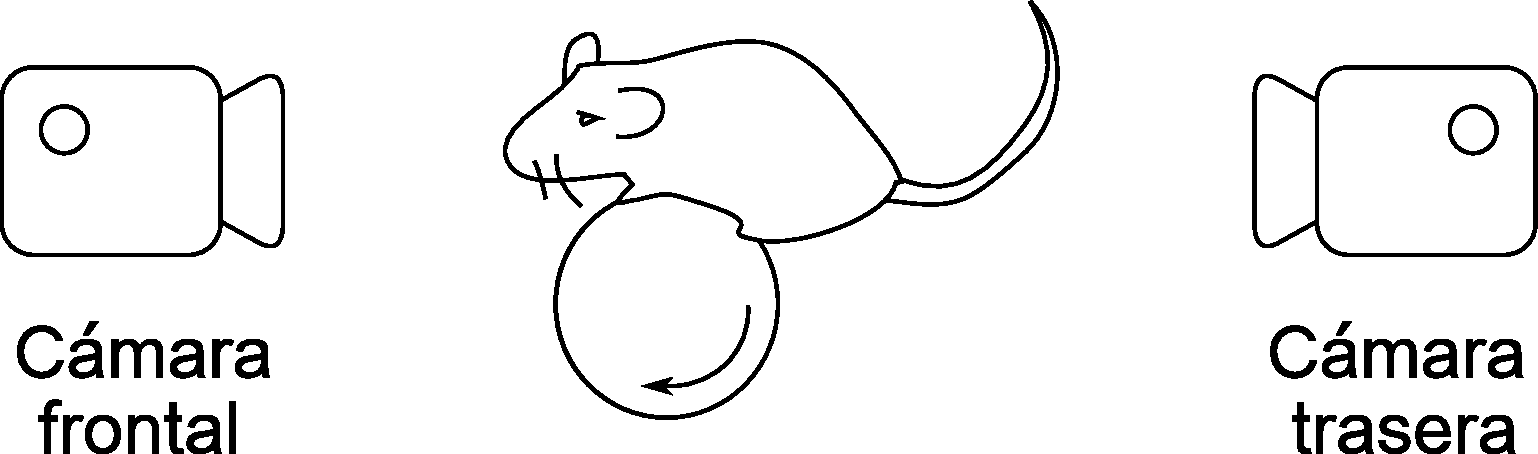
\includegraphics[width=0.55\linewidth]{figuras/capitulo1/camaras.pdf}
    \caption{\textbf{Esquema de cámaras utilizadas.} Cámara frontal, aparato rotarod y cámara trasera.}
    \label{fig:capitulo1_camaras}
\end{figure}